\documentclass[11pt, a4paper, twoside]{article}

% LTeX: language = "es-AR"

% Version en 2024 Víctor Bettachini < vbettachini@unlam.edu.ar >

\usepackage[T1]{fontenc}
\usepackage[utf8]{inputenc}

% \usepackage[spanish, es-tabla]{babel}
% \def\spanishoptions{argentina} % Was macht dass?
% \usepackage{babelbib}
% \selectbiblanguage{spanish}
% \addto\shorthandsspanish{\spanishdeactivate{~<>}}

\usepackage{graphicx}
\graphicspath{{../figuresLaTeX/}}
% \usepackage{float}

\usepackage[arrowdel]{physics}
\newcommand{\pvec}[1]{\vec{#1}\mkern2mu\vphantom{#1}}
% \usepackage{units}
\usepackage[separate-uncertainty= true, multi-part-units= single, range-units= single, range-phrase= {~a~}, locale= FR]{siunitx}
\usepackage{isotope} % $\isotope[A][Z]{X}\to\isotope[A-4][Z-2]{Y}+\isotope[4][2]{\alpha}

\usepackage{tasks}
\usepackage[inline]{enumitem}
% \usepackage{enumerate}

\usepackage{hyperref}

% \usepackage{amsmath}
% \usepackage{amstext}
% \usepackage{amssymb}

\usepackage{tikz}
\usepackage{tikz-3dplot}
\usepackage{tikz-dimline}
\usetikzlibrary{calc}
% \usetikzlibrary{math}
\usetikzlibrary{arrows.meta}
\usetikzlibrary{snakes}
\usetikzlibrary{decorations}
\usetikzlibrary{decorations.pathmorphing}
\usetikzlibrary{patterns}

\usepackage[hmargin=1cm,vmargin=3cm, top= 0.75cm,nohead]{geometry}

\usepackage{lastpage}
\usepackage{fancyhdr}
\pagestyle{fancyplain}
\fancyhf{}
\setlength\headheight{28.7pt} 
\fancyhead[LE, LO]{\textbf{Computational Analytical Mechanics} }
% \fancyhead[LE, LO]{\textbf{Mecánica General} }
\fancyhead[RE, RO]{\href{https://ingenieria.unlam.edu.ar/}{$\vcenter{\hbox{\includegraphics[height=1cm]{ambos.pdf}}}$}}
\fancyfoot{\href{https://creativecommons.org/licenses/by-nc-sa/4.0/}{$\vcenter{\hbox{\includegraphics[height=0.4cm]{by-nc-sa_80x15.pdf}}}$} \href{https://ingenieria.unlam.edu.ar/}{DIIT - UNLaM}}
\fancyfoot[C]{ {\tiny Updated \today} }
\fancyfoot[RO, LE]{Page \thepage/\pageref{LastPage}}
\renewcommand{\headrulewidth}{0pt}
\renewcommand{\footrulewidth}{0pt}




\begin{document}
\begin{center}
  \textsc{\large Euler-Lagrange equation}
\end{center}

\noindent
Exercises marked with (*) have extra difficulty, don't hesitate to ask for help.

\begin{enumerate} 

\item
\textbf{Ideal physical pendulum} [Marion ex. 7.2] \\ 
\textbf{Pendulum with free point of support and double pendulum} [Landau \S5 exs. 1 y 2]\\
Apply the Euler-Lagrange equation to obtain the equations that describe the dynamics of the following systems:
\begin{tasks}(3)
	\task 	\begin{tikzpicture}[scale= 1.3]
  	\draw [arrows=-latex] (-1,2) -> (-1,1) node [above=15, right=2] {\(\vec{g}\)}; % g vertical
		\draw [ultra thick] (-1.5,3) -- (2,3);
		\fill [pattern = north east lines] (-1.5,3) rectangle (2,3.2); % techo
		\draw [dashed] (0,3) -- (0,-.25);	% vertical
		\draw [thick] (0,3) -- +(-60:3) node[midway,above,right=2] {\(\ell\)};	% inclinada +:relativa, -60 grados, longitud 3
		\shade [ball color=black!80] ($(0,3)+(-60:3)$) circle(0.25) node [] {\color{white} $m$};
    %\draw [arrows=-latex] (0,.4) -> (1.25,.4) node [midway, above] {\( \psi \)}; % desplazamiento horizontal
		\draw [arrows=-latex] (0,0) arc [start angle=-90, end angle=-65, radius=3] node [below=12, left=8] {\( \varphi \)};
	\end{tikzpicture}
	\task \includegraphics[height=0.23\textwidth]{figures/landauS52_fig2}
	\task \includegraphics[height=0.23\textwidth]{figures/landauS52_fig1}
\end{tasks}
Result 1c:\\
\(
\ell_{1} \left(\ell_{1} m_{1} \ddot{\varphi}_{1} + \ell_{1} m_{2} \ddot{\varphi}_{1} + \ell_{2} m_{2} \sin{\left(\varphi_{1} - \varphi_{2} \right)} \dot{\varphi}_{2}^{2} + \ell_{2} m_{2} \cos{\left(\varphi_{1} - \varphi_{2} \right)} \ddot{\varphi}_{2} + g m_{1} \sin{\left(\varphi_{1} \right)} + g m_{2} \sin{\left(\varphi_{1} \right)}\right) = 0\\
\ell_{2} m_{2} \left(\ell_{1} \sin{\left(\varphi_{1} - \varphi_{2} \right)} \dot{\varphi}_{1}^{2} - \ell_{1} \cos{\left(\varphi_{1} - \varphi_{2} \right)} \ddot{\varphi}_{1} - \ell_{2} \ddot{\varphi}_{2} - g \sin{\left(\varphi_{2} \right)}\right) = 0
\)


\item
	\begin{minipage}[t][4.5cm]{0.7\textwidth}
		\textbf{Mobile inclined plane}\\
		A block of mass \(m_1\) is initially at rest on an inclined plane \(\theta\) of mass \(M\), without friction between the two bodies.
		The former can slide over the horizontal surface, also without friction.
		Let's call \(c\) the coordinate for the inclined plane, directed as shown in the figure, and \(d\) the coordinate for the block on top.
		\begin{enumerate}
			\item Write the Euler-Lagrange equation for \(c\) and for \(d\).\\ 
			Result:
	\(
		M \ddot{c} - m \cos{\left(\theta \right)} \ddot{d} + m_1 \ddot{c} = 0
		\qquad
		m_1 \left(g \sin{\left(\theta \right)} + \cos{\left(\theta \right)} \ddot{c} - \ddot{d }\right) = 0
	\)
		\end{enumerate}
	\end{minipage}
	\begin{minipage}[c][0cm][t]{0.3\textwidth}
		\begin{tikzpicture}[scale= 1.3]
	% piso
	\draw [ultra thick] (-2,0) -- (1.7,0);
	\fill [pattern = north east lines] (-2,-0.2) rectangle (1.7,0);

	\draw [thick] (-1.5,0) node [above = 0.7 cm, right = 0.4 cm] {\(M\)} -- (-1.5,1.5) -- (1.5,0) -- cycle;
	\draw [arrows=-latex] (0.4,0) ++(0:0.5) arc (0:-33:-0.5) node [midway, left] {\(\theta\)};
	\draw [arrows=-Latex] (-1.6,0.7) -> (-2,0.7) node [midway, above] {\(\vec{c}\)};
	
	% Box sliding down the hypotenuse
	\coordinate (box) at (-0.5,1);
	\draw[thick,rotate around={-26:(box)}] (box) rectangle ++(1,0.5) node [midway] {\(m_1\)};
	% draw circle a a certain distance from (box)
 	\draw [arrows=-Latex, rotate={-26}] (0.3,0.9) -> (0.8,0.9) node [midway, above] {\(\vec{d}\)};
\end{tikzpicture}
	\end{minipage}
	You should notice that you couldn't provide an answer to a question such as ``If the block is realeased, what is the inclined plane's acceleration?'' because this is a coupled differential equations system.
	You will learn how to solve this system using \verb'SymPy' in the next class.


\item
	\begin{minipage}[t][4.5cm]{0.7\textwidth}
		\textbf{Pendulum motion on an inclined plane}\\
		A support of mass \(m_1\) slides on an inclined plane with angle \(\theta\), without friction.
		A pendulum of length \(\ell\) and mass \(m\) hangs from the support making an angle \(\varphi\) with respect to the vertical direction.
		The support protrudes to one side allowing the pendulum to move freely without interference from the inclined plane.
		\begin{enumerate}
			\item Find the dynamic equations for this system.\\
			Result:
			\(
				\ell m \left(\ell \ddot{\varphi} + g \sin{\left(\varphi \right)} + \cos{\left(\theta + \varphi \right)} \ddot{d}\right) = 0 \\
				\ell m \sin{\left(\theta + \varphi \right)} \dot{\varphi}^{2} - \ell m \cos{\left(\theta + \varphi \right)} \ddot{\varphi} + g m \sin{\left(\theta \right)} + g m_{1} \sin{\left(\theta \right)} - m \ddot{d} - m_{1} \ddot{d} = 0
			\)
		\end{enumerate}
	\end{minipage}
	\begin{minipage}[c][0cm][t]{0.3\textwidth}
		\begin{tikzpicture}[scale= 1.3]
	% piso
	\draw [ultra thick] (-2,0) -- (1.7,0);
	\fill [pattern = north east lines] (-2,-0.2) rectangle (1.7,0);

	% plano inclinado
	\draw [thick] (-1.5,0) -- (-1.5,1.5) -- (1.5,0) -- cycle;
	% arc for the angle theta
	\draw [arrows=-latex] (0.4,0) ++(0:0.5) arc (0:-33:-0.5) node [midway, left] {\(\theta\)};
	% \draw [arrows=-Latex] (-1.6,0.7) -> (-2,0.7) node [midway, above] {\(\vec{c}\)};
		
	% Box sliding down the hypotenuse
	\coordinate (box) at (-0.5,1);
	\draw[thick,rotate around={-26:(box)}] (box) rectangle ++(1,0.5) node [midway, below = 1 mm, right= -1 mm] {\(m_1\)};
 	\draw [arrows=-Latex, rotate={-26}] (0.3,0.9) -> (0.8,0.9) node [midway, above] {\(\vec{d}\)};

	\draw [very thick] (box) ++(0.5,0) -- ++(-0.5,-1.7) node [midway, left] {\(\ell\)};
	
	\shade [ball color=black!80] (-0.5,-0.7) circle(0.25) node [] {\color{white} $m$};

	\draw [dashed] (box) ++(0.5,0) -- ++(0,-1.95);
	% arc from the vertical previous very thick line marking angle varphi
	\draw [arrows=-latex] (box) ++(0.5,-1.4)  arc (-90:-99:2.5) node [midway, right= 2 mm] {\(\varphi\)};

\end{tikzpicture}
	\end{minipage}
	


\item
	\begin{minipage}[t][3.9cm]{0.75\textwidth}
		\textbf{Spring coiled around a T-shaped arm}\\
		The T-shaped device shown in the figure is connected by a rod of length \(\ell\) to a pivot point.
		The T spins over an horizontal plane with constant angular speed \(\omega\).
		A particle of mass \(m\) much larger than that of the T (so that the mass of the T can be neglected) can slide freely over the perpendicular arm on the T, attached to the end of a spring of constant \(k\) and zero natural length, that is connected to the joint of the T-arm.
	\end{minipage}
	\begin{minipage}[c][1cm][t]{0.3\textwidth}
		\begin{tikzpicture}
% Define coordinates
\coordinate (O) at (0,0); % Origin point

% Draw a rod at 40 degrees to the horizontal of length 2
\begin{scope}[rotate = 40]
  \draw[very thick] (O) -- (2,0) node[midway, right] {$\ell$};
  \draw[very thick] (2,2) -- (2,-2);
	\shade [ball color=black!80] (2, 1.25) circle(0.25) node [] {\color{white} $m$};
  \draw[decorate, decoration= {coil, amplitude=1.5mm, segment length=1.5 mm}] (2,0) -- (2,1) node[midway,below left] {$k$};
  % \filldraw[black] (2,1.5) circle (1.5mm) node[above right] {$m$};
\end{scope}

% Draw pivot point
\draw[black, fill=white] (O) circle (1.5 mm);
\filldraw[black] (O) circle (0.5 mm);

% arrow around 0 from angle 60 to 120
\draw[-Latex] (.5,0.5) arc (60:120:1) node[midway, above]{\(\omega\)};


\end{tikzpicture}
	\end{minipage}
	\begin{enumerate}
		\item Find a dynamic equation in terms of \(d\), the distance between the particle and the joint.\\
		Result: \(- \omega^{2} m d + k d + m \ddot{d} = 0\)
		\item (*) There exists a ``special value'' for \(\omega\). What is this value and how it relates to \(d(t)\)?
	\end{enumerate}


\end{enumerate}
\end{document}
